% GatiSaarth - IEEE conference paper draft.
% Build: pdflatex gatisaarth_ieee; bibtex gatisaarth_ieee; pdflatex x2
% (or upload this folder to Overleaf; IEEEtran is built in there).
% Figures: python make_figures.py ../evidence/iovnbd_outage_benchmark.json synthetic_and_phone_scores.json
\documentclass[conference]{IEEEtran}
\IEEEoverridecommandlockouts
\usepackage{cite}
\usepackage{amsmath,amssymb}
\usepackage{graphicx}
\usepackage{booktabs}
\usepackage{multirow}
\usepackage{url}
\usepackage{xcolor}
\newcommand{\todo}[1]{\textcolor{red}{[TODO: #1]}}

\begin{document}

\title{Never Worse Than Holding Velocity: Integrity-Gated, Fully Offline Smartphone Dead Reckoning for Vehicular GNSS Outages, and a Reference-Free Way to Test It}

\author{\IEEEauthorblockN{\todo{Author 1}, \todo{Author 2}, \todo{Author 3}}
\IEEEauthorblockA{\todo{Department, Institution, City, India}\\
\todo{email addresses}}}

\maketitle

\begin{abstract}
Phones lose satellite positioning in tunnels, under flyovers and between tall
buildings, exactly where drivers most need a position. Published smartphone
dead-reckoning (DR) methods improve accuracy with better filters or learned
models, but are typically evaluated offline against survey-grade reference
systems, seldom report what a trivial predictor would have achieved, and say
little about what the phone should do when its own estimator is wrong. We present GatiSaarth, an
Android navigation system that runs entirely on the phone, with no server and
no network: a 15-state error-state extended Kalman filter with vehicle-motion
constraints, online phone-to-vehicle mount alignment, heading-only map matching
on vector map packs stored on the device, and a learned forward-speed model that
is admitted only after it agrees with the receiver's Doppler speed. An integrity
gate hands the displayed position to the filter only while the filter is
predicting live fixes at least as well as holding the last velocity, so that,
as far as the live fixes can show, the inertial solution never degrades what
the user sees. We also propose an outage
benchmark that needs no reference receiver: it replays any recorded drive, withholds
the phone's own GNSS for 10--120\,s at many start times, and reports error
against the withheld fixes, the hold-velocity baseline, 3-sigma consistency and
every window it declined to score. On real vehicle trips from the IO-VNBD
dataset (vehicle-grade inertial channels, reference-receiver positions), on the
25 trips where the filter led, its median drift is 12.5\,\% of distance at
60\,s against 57.8\,\% for holding velocity. On a real phone lying loose in an
auto-rickshaw, the gate withheld the filter in 56 of 60 candidate windows,
which kept the displayed position at baseline instead of letting it degrade.
On a 51\,km synthetic Mumbai set the filter wins at 10--30\,s but loses from
60\,s, the opposite of the real trips; we show why that result cannot count as
validation. None of the configurations meets a 10\,\% drift target at
60--120\,s.
\end{abstract}

\begin{IEEEkeywords}
dead reckoning, GNSS outage, smartphone navigation, inertial navigation,
extended Kalman filter, map matching, integrity monitoring, evaluation
methodology
\end{IEEEkeywords}

\section{Introduction}
A consumer phone carries every sensor needed for inertial dead reckoning: a
three-axis accelerometer and gyroscope, a magnetometer and a GNSS receiver that
reports position, Doppler speed and course once per second. When the GNSS
signal disappears in a tunnel, under an elevated road or in a dense urban
canyon, a navigation app typically freezes the marker or extrapolates the last
velocity in a straight line. For Indian cities, where two-wheelers and
auto-rickshaws dominate traffic, flyovers are common, and new tunnels such as
Mumbai's coastal road carry commuters for more than a kilometre underground,
this gap is a daily experience rather than an edge case.

The research literature has attacked the problem from two sides. Model-based
work integrates the phone's MEMS inertial sensors with GNSS in a Kalman filter,
adds vehicle-motion constraints and estimates how the phone sits in the
car~\cite{niu2012iphone,mu2019arbitrary,wang2025velocity}. Learning-based work
trains networks to regress speed, displacement or pseudo-GNSS positions from
inertial windows~\cite{wang2023deepodometry,vishnukumar2026denoiser,shin2025speed,xiao2025speed}
or to tune the filter's noise~\cite{brossard2020aiimu}. Both families report
their accuracy against an instrumented vehicle carrying a reference
system, usually offline, and on data where the phone's mounting was controlled
or augmented.

That leaves three questions unanswered that matter when the system has to run
on a stranger's phone. First, \emph{what does the phone do when its own
estimator is wrong?} A filter with a mis-estimated mount or heading can be
confidently worse than the naive extrapolation it replaced. Second, \emph{can the
method be tested without a reference receiver?} Survey-grade references do not
scale to thousands of phone models and roads. Third, \emph{does the claimed gain
survive a comparison with the simplest possible predictor?} Learned models are
usually compared with a pure inertial solution or a conventional filter, whose
error grows quickly, rather than with holding the last GNSS velocity, which is
what the user would otherwise see.

This paper describes GatiSaarth, a navigation system built around those
questions, and reports what it achieves and where it fails. Our contributions
are:
\begin{enumerate}
\item A complete, fully on-device and offline DR pipeline for Android
(Section~\ref{sec:system}): an error-state EKF with non-holonomic and
zero-velocity updates, online mount alignment from GNSS speed changes,
heading-only HMM map matching and road-locked DR on vector map packs that the
phone itself cuts into a road graph, and a learned forward-speed model that is
admitted only after it agrees with GNSS.
\item An \emph{integrity-gated hand-over} that lets the filter drive the
displayed position only while it has earned it, by predicting the next live
fixes at least as well as holding velocity; otherwise the app keeps its
non-inertial pipeline (Section~\ref{sec:gate}).
\item A \emph{reference-free outage benchmark} that any phone can run on its
own recordings, with a hold-velocity baseline, uncertainty consistency and an
explicit account of every window it did not score (Section~\ref{sec:bench}).
\item An honest evaluation on real vehicle trips, real phone drives and a
labelled synthetic set, including the negative results: where the filter loses
to the baseline, where the learned model is gated out, and why the synthetic
data disagrees with the real data (Sections~\ref{sec:results}--\ref{sec:discussion}).
\end{enumerate}

\section{Related Work and the Gap}
\label{sec:related}

\subsection{Model-based smartphone navigation in vehicles}
Wahlstr{\"o}m \emph{et al.}~\cite{wahlstrom2017telematics} survey a decade of
smartphone vehicle telematics and single out the phone's unknown and changing
orientation in the vehicle as the defining difficulty. Niu
\emph{et al.}~\cite{niu2012iphone} showed early that an iPhone's inertial
sensors can bridge GNSS gaps once the mounting misalignment is estimated. Mu
and Zhao~\cite{mu2019arbitrary} estimate the misalignment of an arbitrarily
mounted device inside a GNSS/INS filter; Wang
\emph{et al.}~\cite{wang2025velocity} make 3-D velocity constraints robust to
mounting angles; learned alternatives estimate the installation angle
directly~\cite{wang2023installangle,freydin2024alignment}. Non-holonomic
constraints (NHC) date back to Dissanayake
\emph{et al.}~\cite{dissanayake2001nhc} and remain central in recent
consistent-robust SINS/GNSS/NHC designs~\cite{du2024nhc}. Steering-wheel
mounted phones~\cite{moussa2019steering} and NavIC-aided low-cost
INS~\cite{sirikonda2021navic,sirikonda2025navic} show the breadth of this line.
These works establish \emph{how} to estimate the state; they evaluate against
reference systems, generally offline.

\subsection{Learned inertial navigation}
Learned inertial odometry began with pedestrians~\cite{chen2018ionet,herath2020ronin,liu2020tlio};
Chen and Pan~\cite{chen2024survey} survey its spread to vehicles. For cars,
networks adapt filter noise~\cite{brossard2020aiimu}, predict position
increments during GPS outages~\cite{liu2021ekfdl,liu2022bridge}, denoise the
IMU~\cite{damagatla2024denoise}, learn wheel-odometry errors on the IO-VNBD
dataset~\cite{onyekpe2021whonet,onyekpe2021iovnbd}, or regress speed and
displacement from phone inertial data~\cite{wang2023deepodometry,shin2025speed,xiao2025speed}.
Vishnukumar \emph{et al.}~\cite{vishnukumar2026denoiser} generate pseudo-GNSS
positions on smartphones with a CNN-GRU after IMU denoising. These methods report
large gains, but typically against a pure inertial or filter-only baseline and
without a runtime test of whether the network's output should be trusted on the
current drive.

\subsection{Map aiding}
Map matching with hidden Markov models~\cite{newson2009hmm} is standard for
snapping traces to roads, and maps have long aided DR, up to lane-level
navigation with enhanced maps~\cite{toledomoreo2009lane}. Mahmoud
\emph{et al.}~\cite{mahmoud2022mapmatch} combine smartphone GNSS, MEMS INS
and HMM map matching for land vehicles in GNSS-denied segments.

\subsection{Integrity and evaluation}
Integrity monitoring for GNSS/INS in automated driving is reviewed
in~\cite{jing2022integrity,viveiros2025integrityai}; it targets protection
levels for safety-critical positioning rather than the question of when a
consumer app should prefer its filter over naive extrapolation. Public
datasets~\cite{onyekpe2021iovnbd,hsu2023urbannav,wang2024whusmartphone,gao2025sensnav,fu2022sdc}
pair phones or low-cost sensors with reference trajectories from instrumented
vehicles. They are indispensable, but their cost limits how many devices,
mounts and cities can be covered. For India, NavIC-capable phones have been
characterised in static and open-sky tests~\cite{kuna2023navic,ainapure2025navic},
not in dynamic outage bridging.

\begin{table*}[t]
\centering
\caption{Representative prior work against the properties this paper targets.
\checkmark: a stated part of the work; --: not described in the paper's
abstract or main contribution (it may exist but is not claimed).}
\label{tab:related}
\begin{tabular}{@{}lcccccc@{}}
\toprule
Work & Phone IMU & Mount handled & Learned part & Map aiding & Runtime trust gate & Reference-free evaluation\\
\midrule
Niu \emph{et al.}~\cite{niu2012iphone} & \checkmark & \checkmark & -- & -- & -- & --\\
Mu \& Zhao~\cite{mu2019arbitrary} & \checkmark & \checkmark & -- & -- & -- & --\\
Wang \emph{et al.}~\cite{wang2025velocity} & \checkmark & \checkmark & -- & -- & -- & --\\
Brossard \emph{et al.}~\cite{brossard2020aiimu} & -- & -- & \checkmark & -- & -- & --\\
Liu \& Guo~\cite{liu2021ekfdl} & -- & -- & \checkmark & -- & -- & --\\
Wang \emph{et al.}~\cite{wang2023deepodometry} & \checkmark & -- & \checkmark & -- & -- & --\\
Vishnukumar \emph{et al.}~\cite{vishnukumar2026denoiser} & \checkmark & -- & \checkmark & -- & -- & --\\
Shin \emph{et al.}~\cite{shin2025speed} & \checkmark & \checkmark & \checkmark & -- & -- & --\\
Mahmoud \emph{et al.}~\cite{mahmoud2022mapmatch} & \checkmark & -- & -- & \checkmark & -- & --\\
Onyekpe \emph{et al.}~\cite{onyekpe2021whonet} & -- & -- & \checkmark & -- & -- & --\\
\midrule
\textbf{This work} & \checkmark & \checkmark & \checkmark (gated) & \checkmark (offline) & \checkmark & \checkmark\\
\bottomrule
\end{tabular}
\end{table*}

\subsection{The gap}
Table~\ref{tab:related} summarises the pattern. One line of work (for example
\cite{wang2023deepodometry,vishnukumar2026denoiser}) makes the estimate better
with learning; another (for example \cite{mu2019arbitrary,wang2025velocity,mahmoud2022mapmatch})
makes it better with constraints, mount estimation and maps. Both assume the
improved estimator should be used whenever it runs, and both are validated
against a reference system that an ordinary user does not have. What neither
provides is (G1) a runtime rule that decides, on the current phone and drive,
whether the inertial solution deserves to be shown at all; (G2) an evaluation
protocol that any phone can execute on its own recordings, with the naive
baseline and abstentions reported alongside accuracy; and (G3) a deployed,
fully offline integration of these pieces that has been measured against its
own failure cases. We found no work in our search that addresses all three for
consumer vehicles; this paper aims to fill that gap. We do not claim a more
accurate estimator than the state of the art.

\section{System}
\label{sec:system}
Fig.~\ref{fig:arch} shows the pipeline. It is written in Dart, runs inside the
Flutter app on Android, and has no server component; recorded drives leave the
phone only through the system share sheet.

\begin{figure*}[t]
\centering
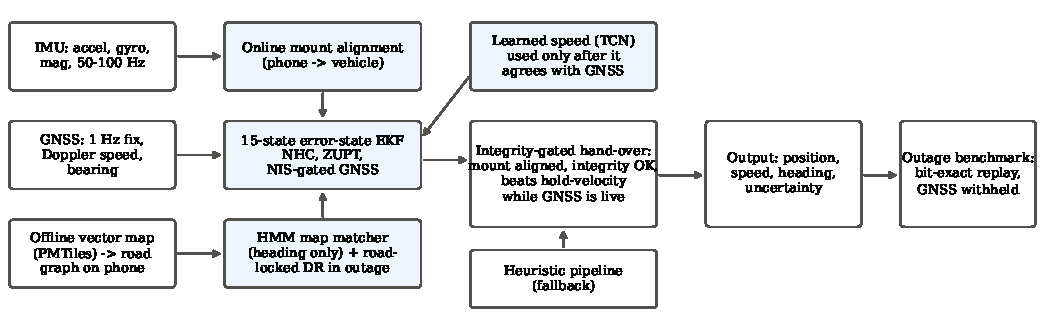
\includegraphics[width=\textwidth]{fig_arch.pdf}
\caption{On-phone pipeline. Shaded blocks form the navigation core; the
integrity gate chooses between its output and the pre-existing heuristic
pipeline. The same code replays recorded drives bit-exactly for the outage
benchmark.}
\label{fig:arch}
\end{figure*}

\subsection{Sensors and time}
Android timestamps inertial samples on the device's uptime clock and GNSS fixes
on the epoch clock. The core integrates on the inertial timeline, so each fix
is stamped with the newest inertial timestamp plus the wall time elapsed since
that sample arrived. Stamping a fix with the inertial time alone collapses the
spacing of queued fixes to milliseconds, and the GNSS gate then rejects them as
teleports; we found this only on real devices.

\subsection{Error-state EKF}
The nominal state holds position, velocity, the body-to-navigation quaternion
and accelerometer and gyroscope biases; the filter estimates a 15-dimensional
error state $\delta\mathbf{x} = [\delta\mathbf{p}, \delta\mathbf{v},
\delta\boldsymbol{\theta}, \delta\mathbf{b}_a, \delta\mathbf{b}_g]$ and feeds
corrections back after every update. Biases follow first-order Gauss--Markov
models. Measurement updates are GNSS position and velocity, zero-velocity
(ZUPT) and zero-angular-rate updates when stationary, non-holonomic constraints
(lateral and vertical vehicle-frame velocity near zero, loosened for
two-wheelers), receiver Doppler speed as a forward-speed update when no course
is available, map heading, and the gated learned speed. Every update is gated
by its normalised innovation squared against the 99\,\% $\chi^2$ quantile.
Covariance updates use the Joseph form with symmetrisation, an eigenvalue floor
and a NaN guard that declares a filter failure instead of emitting a number.

\subsection{Online mount alignment}
The phone-to-vehicle rotation is not known. Gravity fixes two of its three
degrees of freedom; the forward axis is found by regressing the horizontal
specific force on the longitudinal acceleration derived from GNSS speed, using
only straight segments (yaw rate below 0.08\,rad/s) with speed changes above
0.5\,m/s$^2$ where the two instruments agree within a factor of 0.4--2.5. The
fit is accepted only after at least 20 distinct speed-change events and 400
samples, a regression $R^2 \geq 0.45$ and a confidence of 0.6; it restarts if
the gravity direction in the phone frame moves by more than 0.25\,rad, which
means the phone has moved in its holder. In practice this needs about 40\,s of
accelerating and braking on straight road.

\subsection{Heading from GNSS}
Some receivers never report a bearing. The core therefore derives a course from
chords of at least 20\,m between fixes, waits for a heading before it
initialises, and re-seeds itself when the GNSS course keeps disagreeing with
the filter. We added this after a real drive in which a wrong initial heading
sealed itself in: NHC pinned velocity along the wrong axis, speed collapsed and
yaw became unobservable, while the filter reported high integrity.

\subsection{Offline maps and road-locked DR}
Maps are vector PMTiles packs downloaded once per region (for example 25.7\,MB
for Mumbai). The phone decodes road geometry for the area around the vehicle,
nodes it at junctions and builds a road graph locally. An HMM matcher in the
style of~\cite{newson2009hmm} runs over a sliding window of fused positions and
reports a match only when one road exceeds a posterior of 0.6 and beats the
runner-up by a margin. The match feeds back only a soft \emph{heading}
measurement; position is never snapped into the filter state. During an outage
a road follower advances the marker along the matched road and uses the gyro
to choose at junctions; a live GNSS fix always releases the lock.

\subsection{Gated learned forward speed}
A residual dilated causal temporal convolutional network (48\,770 parameters,
a 209\,KB TensorFlow Lite model with built-in operators only) regresses forward
speed and its variance from 2\,s windows (20 samples at 10\,Hz) of 13 features
of levelled vehicle-frame accelerometer and gyroscope data. It was trained from
scratch with a $\beta$-NLL loss on 341\,736 windows of real IO-VNBD trips with
reference-receiver speed labels; on held-out trips its mean absolute error is
3.33\,m/s with 61\,\% of errors inside one predicted sigma. The model enters the filter only after its output
has agreed with the receiver's Doppler speed on the current drive with an RMS
difference of at most 1\,m/s, and it is rejected whenever it disagrees with the
inertial forward speed by more than four combined sigmas.

\subsection{Integrity-gated hand-over}
\label{sec:gate}
The app had a heuristic pipeline (GNSS when live, heading-and-speed
extrapolation otherwise) before the core existed. The core's solution replaces
it only while all of the following hold: the mount alignment has converged;
the integrity monitor is not in its invalid state and the filter is
numerically healthy; the minimum sensor set is present; and, while GNSS is
live, the core has \emph{earned trust}. Earned trust compares, over the last
20 fixes, the median distance between each new fix and the core's prediction
of it with the same quantity for holding the last velocity, and requires
\begin{equation}
\operatorname{med}_{20}\!\left(e_{\mathrm{core}}\right) \le
1.25\,\operatorname{med}_{20}\!\left(e_{\mathrm{hold}}\right) + 2\,\mathrm{m}.
\end{equation}
If any condition fails the app hands back to its heuristic pipeline at once.
A regression test pins the resulting property: with the core present the app
can never show a worse position than it did before the core existed, under
the conditions the gate can observe.

\section{Reference-Free Outage Benchmark}
\label{sec:bench}
The benchmark replays a recorded drive through exactly the code that runs
live; replay is bit-exact, so a change in the numbers is attributable to a code
change. At 17 start times spread over the drive it withholds GNSS for 10, 30,
60 and 120\,s and compares, at the end of the blackout, the core's position
with the fix the phone actually recorded there. Fixes serve as truth only
if their reported accuracy passes a quality filter, and the report states the
truth's median accuracy as its noise floor. For each blackout length it
reports the median and 95th-percentile error, drift as error divided by the
distance travelled during the blackout, the same numbers for holding the last
velocity, how often the core was closer than the baseline, and how often the
real error fell inside the core's own 3-sigma bound. A window is scored only if
the gate would have let the core lead at its start; every other window is
counted with its reason (core not leading, no recent fix, no truth at the end,
too little travel).

The design trades absolute truth for reach. Its truth is only as good as the
phone's GNSS (3--10\,m median in our drives), so it cannot resolve errors below
that floor and is not a substitute for a reference receiver when one exists.
In exchange it runs on any recording from any phone, which is the only way we
know to measure performance on the devices and roads the product will meet.

\section{Experimental Setup}
\label{sec:setup}

\begin{table}[t]
\centering
\caption{Data used in the evaluation.}
\label{tab:data}
\begin{tabular}{@{}p{2.1cm}p{5.8cm}@{}}
\toprule
Set & Description\\
\midrule
IO-VNBD (real) & 32 trips $\geq$5\,min, Coventry, UK~\cite{onyekpe2021iovnbd}. Inertial input: the vehicle's own ESP/CAN longitudinal and lateral acceleration and yaw rate at 10\,Hz (a vehicle-grade external IMU proxy, not a phone IMU); GNSS and truth: Racelogic VBOX at 1\,Hz.\\
Phone drives (real) & 4 drives, Mumbai, Sept.\ 2026, realme RMX3851 and RMX5264, 100\,Hz IMU, 1\,Hz GNSS. Phones hand-held or lying loose (one on an auto-rickshaw seat); no rigid holder.\\
Perturbed copies (derived) & 5 copies of the 10.6\,min rickshaw drive with small noise added to every channel and some fixes dropped.\\
Synthetic Mumbai (synthetic) & 5 generated drives, 51.2\,km, 90.8\,min, 50\,Hz IMU, 1\,Hz GNSS, five phone-model profiles. \todo{Describe the generator: trajectory source, road network, IMU error model, GNSS error model, and how it was validated.}\\
\bottomrule
\end{tabular}
\end{table}

Table~\ref{tab:data} lists the data. IO-VNBD's smartphone accelerometer cannot
be aligned to the vehicle (its sampling is aliased and a gyro column is
mislabelled), so on that dataset the core consumes the vehicle's own inertial
channels; results there measure the estimator and its constraints, not a
phone's sensors. All numbers are from the configuration that ships in the app
(\texttt{NavConfig.live}) unless stated, replayed with the car settings;
``+map'' adds the road graph cut from the region's map pack. Scripts that
reproduce every table are in the project repository.

\section{Results}
\label{sec:results}

\subsection{Real vehicle trips (IO-VNBD)}
Table~\ref{tab:iovnbd} and Fig.~\ref{fig:drift}(a) summarise the 32 trips. The
core led on 27 of them, and 23--26 trips have scored windows at each blackout
length; on the others the filter never became healthy enough to lead, and
those windows are not scored. Re-running the benchmark on the current code
reproduced the stored result file byte for byte. Where it led, the core's median
drift was a quarter or less of the baseline's at every blackout length, and
below 10\,\% on most trips up to 30\,s. At 60\,s it met 10\,\% on 10 of 25
trips, at 120\,s on 1 of 23.

\begin{table}[t]
\centering
\caption{IO-VNBD: median over trips of each trip's median drift (\% of
distance travelled in the blackout).}
\label{tab:iovnbd}
\begin{tabular}{@{}rrrrr@{}}
\toprule
Blackout & Trips & Core & Hold velocity & Trips with core $<$10\,\%\\
\midrule
10\,s & 26 & 4.6 & 18.0 & 22\\
30\,s & 25 & 8.6 & 36.3 & 13\\
60\,s & 25 & 12.5 & 57.8 & 10\\
120\,s & 23 & 18.4 & 68.8 & 1\\
\bottomrule
\end{tabular}
\end{table}

\begin{figure}[t]
\centering
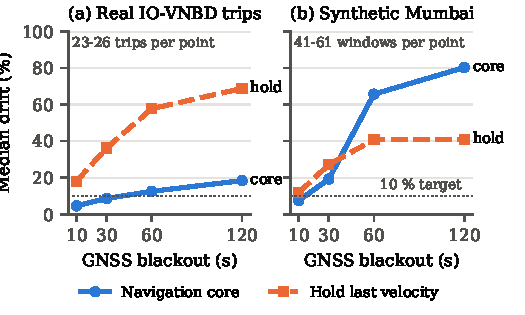
\includegraphics[width=\columnwidth]{fig_drift.pdf}
\caption{Median drift against blackout length. (a) Real IO-VNBD trips (median
over trips). (b) Synthetic Mumbai drives without the map (median over drives).
The dotted line is the 10\,\% target.}
\label{fig:drift}
\end{figure}

\subsection{Real phone drives: the gate at work}
None of the four phone drives came from a phone in a rigid holder, which is
the condition the mounted filter is built for. On the three drives of 24
September the mount alignment never converged, so the core never led and the
app showed its heuristic output throughout. On the 26 September auto-rickshaw
drive the alignment converged after 205\,s, but the earned-trust test failed
almost everywhere: of 60 candidate windows, 56 were withheld because the core
was not allowed to lead. In the four it did lead, it was worse than holding
velocity at 10--60\,s and slightly better at 120\,s
(Table~\ref{tab:phone}). Before the earned-trust test existed, the same drive
had the core leading from 64\,s while 272\,m off at 10\,s against 5.6\,m for
holding velocity. The gate therefore did the job it exists for; it did not
make the loose phone accurate.

\begin{table}[t]
\centering
\caption{Real rickshaw drive (26 Sept.), windows the gate allowed (one per
blackout length). Median error at the end of the blackout, metres.}
\label{tab:phone}
\begin{tabular}{@{}rrrr@{}}
\toprule
Blackout & Hold velocity & Core & Core + map\\
\midrule
10\,s & 4.3 & 26.3 & 20.0\\
30\,s & 16.7 & 45.4 & 48.1\\
60\,s & 131.3 & 162.6 & 142.0\\
120\,s & 538.8 & 561.3 & 473.6\\
\midrule
\multicolumn{4}{@{}l}{Windows withheld by the gate: 56 of 60}\\
\bottomrule
\end{tabular}
\end{table}

The five perturbed copies of that drive probe how close to its acceptance
thresholds the alignment was. Two copies aligned and scored as the original
did; one aligned but scored only with the map; two never aligned. Changes far
smaller than the sensors' own noise flipped a loosely placed phone between
``aligned'' and ``not aligned''.

For phones that are not in a holder at all, the core has an experimental
hand-held mode, off by default: a small kinematic tracker that integrates a
bias-corrected, orientation-invariant yaw rate (the gyro projected on gravity)
at the last GNSS speed, detects stops from the spread of the accelerometer
norm, and takes road heading from the map matcher, with no forward axis and
therefore no NHC. Table~\ref{tab:handheld} scores it on all four phone drives.
With the map it beats holding velocity at 60\,s on two of the four drives and
at 120\,s on two, and is far worse on the short drive A, where the gate also
withheld it in 44 of 52 windows. Its constants were tuned on drives A--C, so
these numbers are optimistic, and the mode stays off in the shipped app.

\begin{table}[t]
\centering
\caption{Experimental hand-held mode on the four real phone drives. Median
error at the end of the blackout (m), 30\,/\,60\,/\,120\,s.}
\label{tab:handheld}
\setlength{\tabcolsep}{2.5pt}
\begin{tabular}{@{}lrlll@{}}
\toprule
Drive & min & Hold velocity & Hand-held & Hand-held + map\\
\midrule
A ($n{=}2$) & 5.7 & 19 / 141 / 177 & 103 / 263 / 664 & 107 / 271 / 669\\
B ($n{=}12$--15) & 7.6 & 60 / 156 / 328 & 69 / 204 / 426 & \textbf{45} / \textbf{140} / 439\\
C ($n{=}11$--15) & 15.4 & 90 / 182 / 403 & 122 / 155 / 250 & \textbf{89} / \textbf{102} / \textbf{241}\\
D ($n{=}2$) & 10.6 & 73 / 211 / 657 & 104 / 287 / 598 & 104 / 287 / \textbf{597}\\
\bottomrule
\end{tabular}
\end{table}

\subsection{Synthetic Mumbai drives}
Table~\ref{tab:synth} and Fig.~\ref{fig:drift}(b) report the synthetic set. The
core led on all five drives after 217--301\,s. It was clearly better than
holding velocity at 10\,s (median 5.4\,m against 12.8\,m, closer in 45 of 61
windows) and still slightly ahead at 30\,s, but from 60\,s it was worse:
at 120\,s its median error was 721\,m against 396\,m, and its 3-sigma bound
held in only 1 of 41 windows. The road graph helped at 60--120\,s and hurt at
30\,s, and did not change the ordering.

\begin{table}[t]
\centering
\caption{Synthetic Mumbai set: median over the five drives of each drive's
median error (m) and drift (\%); ``closer'' and ``$3\sigma$'' count windows.}
\label{tab:synth}
\setlength{\tabcolsep}{3pt}
\begin{tabular}{@{}lrrrrrr@{}}
\toprule
 & Blackout & $n$ & Hold & Core & Closer & $3\sigma$ ok\\
\midrule
\multirow{4}{*}{No map} & 10\,s & 61 & 12.8 (11.8\,\%) & 5.4 (7.5\,\%) & 45 & 58\\
 & 30\,s & 53 & 75.7 (27.1\,\%) & 43.2 (19.2\,\%) & 28 & 40\\
 & 60\,s & 49 & 191.9 (40.8\,\%) & 332.7 (65.7\,\%) & 15 & 13\\
 & 120\,s & 41 & 396.0 (41.0\,\%) & 720.8 (80.3\,\%) & 6 & 1\\
\midrule
\multirow{4}{*}{+ map} & 10\,s & 61 & 12.8 (11.8\,\%) & 5.4 (7.6\,\%) & 41 & 58\\
 & 30\,s & 53 & 75.7 (27.1\,\%) & 62.5 (26.3\,\%) & 22 & 36\\
 & 60\,s & 48 & 220.6 (42.4\,\%) & 279.6 (57.3\,\%) & 17 & 18\\
 & 120\,s & 41 & 396.0 (41.0\,\%) & 677.3 (59.7\,\%) & 9 & 3\\
\bottomrule
\end{tabular}
\end{table}

\subsection{Other measurements}
\emph{Learned speed.} On the held-out IO-VNBD trips the TCN never reaches the
1\,m/s agreement with GNSS Doppler speed that the gate requires, so replays
with the model enabled are identical to replays without it; we claim no drift
reduction from it.

\emph{Ablation (simulated).} On five seeded simulated drives with a 60\,s
blackout, a pure inertial solution drifts 35.1\,\%, adding GNSS velocity
reduces this to 15.4\,\%, and adding NHC to 1.4\,\%; ZUPT and map heading do
not move the number on these cruising profiles. NHC is the dominant lever by an
order of magnitude. These are simulations and bound the estimator under
modelled sensor error; they are not field accuracy.

\emph{Cost.} The core takes about 20\,$\mu$s per sensor frame (74\,$\mu$s
peak) in our replay harness, around 0.1\,\% of one core at 50\,Hz.

\section{Discussion}
\label{sec:discussion}

\subsection{Why the synthetic results disagree with the real trips}
On real IO-VNBD trips the core's advantage over holding velocity grows with the
blackout length; on the synthetic set it shrinks and reverses from 60\,s. Two
explanations fit, and our data cannot separate them. The first is the
generator: if the synthetic accelerometer and gyro are not the physical
derivatives of the synthetic trajectory, an inertial filter is integrating
signals that do not describe the motion. One diagnostic points that way without
settling it: over 4\,s windows while moving, the correlation between the change
in GNSS course and the integrated gyro rate about gravity is 0.46 on the real
rickshaw drive but ranges from 0.03 to 0.51 across the five synthetic drives,
although their GNSS is cleaner (median accuracy 3--5\,m against 10\,m); that
correlation does not, however, track which synthetic drives score worst. The
second explanation is the sensor path: IO-VNBD feeds the core vehicle-frame
inertial channels that need no mount alignment, whereas the synthetic drives,
like a real phone, go through the alignment, and a small residual
misalignment leaks gravity and braking into the forward and lateral axes,
an error that grows with blackout length. If that is the cause, the synthetic
result is a genuine warning about the phone path. Either way the synthetic set
is not validation evidence: we report it as a stress test, and the question it
raises can only be answered by real drives with a rigidly held phone and a
reference receiver. Synthetic drives are useful for exercising code paths, but
must themselves be validated against real recordings before they are used to
judge accuracy.

\subsection{What the gate does and does not guarantee}
The earned-trust test uses the only truth available at run time, the live
fixes, so it protects the transition into an outage and the first seconds of
it, where the prediction is closest to what was just verified. It cannot know
how the error will grow during a long blackout. The 3-sigma column of
Table~\ref{tab:synth} shows the same limit from the other side: the
covariance contains the real error in 58 of 61 windows at 10\,s but in 1 of 41
at 120\,s, so it is over-confident exactly where an honest uncertainty matters
most.

\subsection{Threats to validity}
The phone-sensor evidence comes from four drives in one city on two phone
models, none rigidly mounted; it demonstrates the gate, not phone-IMU accuracy.
IO-VNBD supplies real trajectories but a vehicle-grade inertial proxy. The
hand-held parameters were tuned on the same three drives they are reported on.
The benchmark's truth is the phone's GNSS, whose multipath errors in urban
Mumbai inflate every number, for the core and the baseline alike. Windows the
core did not lead are excluded from its accuracy; we report their count so the
exclusion is visible.

\section{Conclusion}
GatiSaarth shows that a complete inertial dead-reckoning stack with map aiding
and a learned component can run entirely offline on a phone at negligible cost,
and that the right question for such a stack is not only how accurate it is but
when it deserves to be shown. On real vehicle trips its filter keeps drift to
a quarter or less of the naive baseline, without meeting a 10\,\% target beyond
30\,s; on real phones placed loosely, the integrity gate correctly declined to
use it. The reference-free benchmark made both findings measurable without a
reference receiver, and exposed a synthetic dataset that would otherwise have
been mistaken for validation. The next steps are drives with the phone in a
rigid holder alongside a reference receiver, two-wheeler drives, NavIC-enabled
phones, and a covariance that stays honest over long blackouts.

\section*{Data and Code Availability}
\todo{State where the code, the benchmark and the drive logs can be obtained;
note that raw drive logs are full location traces and must be shared with the
drivers' consent.}

\section*{Acknowledgment}
\todo{Acknowledgments.} The IO-VNBD dataset was provided by Onyekpe
\emph{et al.}~\cite{onyekpe2021iovnbd}.

\bibliographystyle{IEEEtran}
\bibliography{references}

\end{document}
